The Drift Tubes (DTs) are a CMS muon system located exclusively in the barrel portion of CMS. They function in a similar way to the CSCs and RPCs, as they detect muons via the direct ionization of a gaseous mixture. A diagram of a DT is shown in Figure \ref{fig:DT_Diagram}. 

\begin{figure}[H]
    \centering
    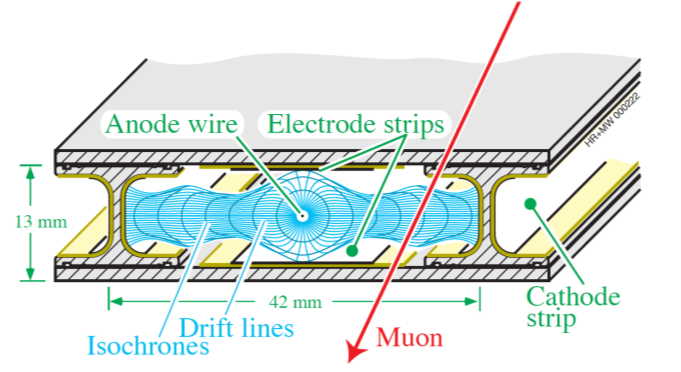
\includegraphics[width=0.7\textwidth]{Images/CMS/Muons/DT/DT_diagram.png}
    \caption{Drift tube diagram}
    \label{fig:DT_Diagram}
\end{figure}

